%% bare_conf.tex
%% V1.3
%% 2007/01/11
%% by Michael Shell
%% See:
%% http://www.michaelshell.org/
%% for current contact information.
%%
%% This is a skeleton file demonstrating the use of IEEEtran.cls
%% (requires IEEEtran.cls version 1.7 or later) with an IEEE conference paper.
%%
%% Support sites:
%% http://www.michaelshell.org/tex/ieeetran/
%% http://www.ctan.org/tex-archive/macros/latex/contrib/IEEEtran/
%% and
%% http://www.ieee.org/

%%*************************************************************************
%% Legal Notice:
%% This code is offered as-is without any warranty either expressed or
%% implied; without even the implied warranty of MERCHANTABILITY or
%% FITNESS FOR A PARTICULAR PURPOSE! 
%% User assumes all risk.
%% In no event shall IEEE or any contributor to this code be liable for
%% any damages or losses, including, but not limited to, incidental,
%% consequential, or any other damages, resulting from the use or misuse
%% of any information contained here.
%%
%% All comments are the opinions of their respective authors and are not
%% necessarily endorsed by the IEEE.
%%
%% This work is distributed under the LaTeX Project Public License (LPPL)
%% ( http://www.latex-project.org/ ) version 1.3, and may be freely used,
%% distributed and modified. A copy of the LPPL, version 1.3, is included
%% in the base LaTeX documentation of all distributions of LaTeX released
%% 2003/12/01 or later.
%% Retain all contribution notices and credits.
%% ** Modified files should be clearly indicated as such, including  **
%% ** renaming them and changing author support contact information. **
%%
%% File list of work: IEEEtran.cls, IEEEtran_HOWTO.pdf, bare_adv.tex,
%%                    bare_conf.tex, bare_jrnl.tex, bare_jrnl_compsoc.tex
%%*************************************************************************

% *** Authors should verify (and, if needed, correct) their LaTeX system  ***
% *** with the testflow diagnostic prior to trusting their LaTeX platform ***
% *** with production work. IEEE's font choices can trigger bugs that do  ***
% *** not appear when using other class files.                            ***
% The testflow support page is at:
% http://www.michaelshell.org/tex/testflow/



% Note that the a4paper option is mainly intended so that authors in
% countries using A4 can easily print to A4 and see how their papers will
% look in print - the typesetting of the document will not typically be
% affected with changes in paper size (but the bottom and side margins will).
% Use the testflow package mentioned above to verify correct handling of
% both paper sizes by the user's LaTeX system.
%
% Also note that the "draftcls" or "draftclsnofoot", not "draft", option
% should be used if it is desired that the figures are to be displayed in
% draft mode.
%
\documentclass[conference,10pt]{IEEEtran}
% Add the compsoc option for Computer Society conferences.
%
% If IEEEtran.cls has not been installed into the LaTeX system files,
% manually specify the path to it like:
% \documentclass[conference]{../sty/IEEEtran}


% Custom packages.
\usepackage{filecontents}
\usepackage{csvsimple}
\usepackage{url}
\newcommand{\var}[1]{$\mathtt{#1}$}



% Some very useful LaTeX packages include:
% (uncomment the ones you want to load)


% *** MISC UTILITY PACKAGES ***
%
%\usepackage{ifpdf}
% Heiko Oberdiek's ifpdf.sty is very useful if you need conditional
% compilation based on whether the output is pdf or dvi.
% usage:
% \ifpdf
%   % pdf code
% \else
%   % dvi code
% \fi
% The latest version of ifpdf.sty can be obtained from:
% http://www.ctan.org/tex-archive/macros/latex/contrib/oberdiek/
% Also, note that IEEEtran.cls V1.7 and later provides a builtin
% \ifCLASSINFOpdf conditional that works the same way.
% When switching from latex to pdflatex and vice-versa, the compiler may
% have to be run twice to clear warning/error messages.






% *** CITATION PACKAGES ***
%
%\usepackage{cite}
% cite.sty was written by Donald Arseneau
% V1.6 and later of IEEEtran pre-defines the format of the cite.sty package
% \cite{} output to follow that of IEEE. Loading the cite package will
% result in citation numbers being automatically sorted and properly
% "compressed/ranged". e.g., [1], [9], [2], [7], [5], [6] without using
% cite.sty will become [1], [2], [5]--[7], [9] using cite.sty. cite.sty's
% \cite will automatically add leading space, if needed. Use cite.sty's
% noadjust option (cite.sty V3.8 and later) if you want to turn this off.
% cite.sty is already installed on most LaTeX systems. Be sure and use
% version 4.0 (2003-05-27) and later if using hyperref.sty. cite.sty does
% not currently provide for hyperlinked citations.
% The latest version can be obtained at:
% http://www.ctan.org/tex-archive/macros/latex/contrib/cite/
% The documentation is contained in the cite.sty file itself.
\usepackage{cite}




% \usepackage{graphicx}
% *** GRAPHICS RELATED PACKAGES ***
%
\ifCLASSINFOpdf
  % \usepackage[pdftex]{graphicx}
  % I don't know... trying to solve bounding box \usepackage{auto-pst-pdf}
  % \usepackage{epstopdf}
  % declare the path(s) where your graphic files are
  % \graphicspath{{../pdf/}{../jpeg/}}
  % and their extensions so you won't have to specify these with
  % every instance of \includegraphics
  % \DeclareGraphicsExtensions{.pdf,.jpeg,.png}
\else
  % or other class option (dvipsone, dvipdf, if not using dvips). graphicx
  % will default to the driver specified in the system graphics.cfg if no
  % driver is specified.
  \usepackage[dvips]{graphicx}
  % declare the path(s) where your graphic files are
  % \graphicspath{{../eps/}}
  % and their extensions so you won't have to specify these with
  % every instance of \includegraphics
  % \DeclareGraphicsExtensions{.eps}
\fi
% graphicx was written by David Carlisle and Sebastian Rahtz. It is
% required if you want graphics, photos, etc. graphicx.sty is already
% installed on most LaTeX systems. The latest version and documentation can
% be obtained at: http://www.ctan.org/tex-archive/macros/latex/required/graphics/
% Another good source of documentation is "Using Imported Graphics in
% LaTeX2e" by Keith Reckdahl which can be found as epslatex.ps or
% epslatex.pdf at: http://www.ctan.org/tex-archive/info/
%
% latex, and pdflatex in dvi mode, support graphics in encapsulated
% postscript (.eps) format. pdflatex in pdf mode supports graphics
% in .pdf, .jpeg, .png and .mps (metapost) formats. Users should ensure
% that all non-photo figures use a vector format (.eps, .pdf, .mps) and
% not a bitmapped formats (.jpeg, .png). IEEE frowns on bitmapped formats
% which can result in "jaggedy"/blurry rendering of lines and letters as
% well as large increases in file sizes.
%
% You can find documentation about the pdfTeX application at:
% http://www.tug.org/applications/pdftex





% *** MATH PACKAGES ***
%
%\usepackage[cmex10]{amsmath}
% A popular package from the American Mathematical Society that provides
% many useful and powerful commands for dealing with mathematics. If using
% it, be sure to load this package with the cmex10 option to ensure that
% only type 1 fonts will utilized at all point sizes. Without this option,
% it is possible that some math symbols, particularly those within
% footnotes, will be rendered in bitmap form which will result in a
% document that can not be IEEE Xplore compliant!
%
% Also, note that the amsmath package sets \interdisplaylinepenalty to 10000
% thus preventing page breaks from occurring within multiline equations. Use:
%\interdisplaylinepenalty=2500
% after loading amsmath to restore such page breaks as IEEEtran.cls normally
% does. amsmath.sty is already installed on most LaTeX systems. The latest
% version and documentation can be obtained at:
% http://www.ctan.org/tex-archive/macros/latex/required/amslatex/math/





% *** SPECIALIZED LIST PACKAGES ***
%
%\usepackage{algorithmic}
% algorithmic.sty was written by Peter Williams and Rogerio Brito.
% This package provides an algorithmic environment fo describing algorithms.
% You can use the algorithmic environment in-text or within a figure
% environment to provide for a floating algorithm. Do NOT use the algorithm
% floating environment provided by algorithm.sty (by the same authors) or
% algorithm2e.sty (by Christophe Fiorio) as IEEE does not use dedicated
% algorithm float types and packages that provide these will not provide
% correct IEEE style captions. The latest version and documentation of
% algorithmic.sty can be obtained at:
% http://www.ctan.org/tex-archive/macros/latex/contrib/algorithms/
% There is also a support site at:
% http://algorithms.berlios.de/index.html
% Also of interest may be the (relatively newer and more customizable)
% algorithmicx.sty package by Szasz Janos:
% http://www.ctan.org/tex-archive/macros/latex/contrib/algorithmicx/




% *** ALIGNMENT PACKAGES ***
%
%\usepackage{array}
% Frank Mittelbach's and David Carlisle's array.sty patches and improves
% the standard LaTeX2e array and tabular environments to provide better
% appearance and additional user controls. As the default LaTeX2e table
% generation code is lacking to the point of almost being broken with
% respect to the quality of the end results, all users are strongly
% advised to use an enhanced (at the very least that provided by array.sty)
% set of table tools. array.sty is already installed on most systems. The
% latest version and documentation can be obtained at:
% http://www.ctan.org/tex-archive/macros/latex/required/tools/


%\usepackage{mdwmath}
%\usepackage{mdwtab}
% Also highly recommended is Mark Wooding's extremely powerful MDW tools,
% especially mdwmath.sty and mdwtab.sty which are used to format equations
% and tables, respectively. The MDWtools set is already installed on most
% LaTeX systems. The lastest version and documentation is available at:
% http://www.ctan.org/tex-archive/macros/latex/contrib/mdwtools/


% IEEEtran contains the IEEEeqnarray family of commands that can be used to
% generate multiline equations as well as matrices, tables, etc., of high
% quality.


%\usepackage{eqparbox}
% Also of notable interest is Scott Pakin's eqparbox package for creating
% (automatically sized) equal width boxes - aka "natural width parboxes".
% Available at:
% http://www.ctan.org/tex-archive/macros/latex/contrib/eqparbox/





% *** SUBFIGURE PACKAGES ***
\usepackage[tight,footnotesize]{subfigure}
% subfigure.sty was written by Steven Douglas Cochran. This package makes it
% easy to put subfigures in your figures. e.g., "Figure 1a and 1b". For IEEE
% work, it is a good idea to load it with the tight package option to reduce
% the amount of white space around the subfigures. subfigure.sty is already
% installed on most LaTeX systems. The latest version and documentation can
% be obtained at:
% http://www.ctan.org/tex-archive/obsolete/macros/latex/contrib/subfigure/
% subfigure.sty has been superceeded by subfig.sty.



%\usepackage[caption=false]{caption}
%\usepackage[font=footnotesize]{subfig}
% subfig.sty, also written by Steven Douglas Cochran, is the modern
% replacement for subfigure.sty. However, subfig.sty requires and
% automatically loads Axel Sommerfeldt's caption.sty which will override
% IEEEtran.cls handling of captions and this will result in nonIEEE style
% figure/table captions. To prevent this problem, be sure and preload
% caption.sty with its "caption=false" package option. This is will preserve
% IEEEtran.cls handing of captions. Version 1.3 (2005/06/28) and later (recommended due to many 
% improvements over 1.2) of subfig.sty supports
% the caption=false option directly:
%\usepackage[caption=false,font=footnotesize]{subfig}
%
% The latest version and documentation can be obtained at:
% http://www.ctan.org/tex-archive/macros/latex/contrib/subfig/
% The latest version and documentation of caption.sty can be obtained at:
% http://www.ctan.org/tex-archive/macros/latex/contrib/caption/




% *** FLOAT PACKAGES ***
%
\usepackage{fixltx2e}
% fixltx2e, the successor to the earlier fix2col.sty, was written by
% Frank Mittelbach and David Carlisle. This package corrects a few problems
% in the LaTeX2e kernel, the most notable of which is that in current
% LaTeX2e releases, the ordering of single and double column floats is not
% guaranteed to be preserved. Thus, an unpatched LaTeX2e can allow a
% single column figure to be placed prior to an earlier double column
% figure. The latest version and documentation can be found at:
% http://www.ctan.org/tex-archive/macros/latex/base/



%\usepackage{stfloats}
% stfloats.sty was written by Sigitas Tolusis. This package gives LaTeX2e
% the ability to do double column floats at the bottom of the page as well
% as the top. (e.g., "\begin{figure*}[!b]" is not normally possible in
% LaTeX2e). It also provides a command:
%\fnbelowfloat
% to enable the placement of footnotes below bottom floats (the standard
% LaTeX2e kernel puts them above bottom floats). This is an invasive package
% which rewrites many portions of the LaTeX2e float routines. It may not work
% with other packages that modify the LaTeX2e float routines. The latest
% version and documentation can be obtained at:
% http://www.ctan.org/tex-archive/macros/latex/contrib/sttools/
% Documentation is contained in the stfloats.sty comments as well as in the
% presfull.pdf file. Do not use the stfloats baselinefloat ability as IEEE
% does not allow \baselineskip to stretch. Authors submitting work to the
% IEEE should note that IEEE rarely uses double column equations and
% that authors should try to avoid such use. Do not be tempted to use the
% cuted.sty or midfloat.sty packages (also by Sigitas Tolusis) as IEEE does
% not format its papers in such ways.





% *** PDF, URL AND HYPERLINK PACKAGES ***
%
%\usepackage{url}
% url.sty was written by Donald Arseneau. It provides better support for
% handling and breaking URLs. url.sty is already installed on most LaTeX
% systems. The latest version can be obtained at:
% http://www.ctan.org/tex-archive/macros/latex/contrib/misc/
% Read the url.sty source comments for usage information. Basically,
% \url{my_url_here}.





% *** Do not adjust lengths that control margins, column widths, etc. ***
% *** Do not use packages that alter fonts (such as pslatex).         ***
% There should be no need to do such things with IEEEtran.cls V1.6 and later.
% (Unless specifically asked to do so by the journal or conference you plan
% to submit to, of course. )


% correct bad hyphenation here
% \hyphenation{op-tical net-works semi-conduc-tor}


\begin{document}
%
% paper title
% can use linebreaks \\ within to get better formatting as desired
\title{GPU Encrypt: AES Encryption on Mobile Devices}


% author names and affiliations
% use a multiple column layout for up to three different
% affiliations
\author{\IEEEauthorblockN{James Gleeson, Sreekumar Rajan, Vandana Saini}
\IEEEauthorblockA{Department of\\Computer Science\\
University of Toronto\\
Toronto, ON\\
\{jagleeso,sreekumar.rajan,vsaini\}@cs.toronto.edu}
}

% conference papers do not typically use \thanks and this command
% is locked out in conference mode. If really needed, such as for
% the acknowledgment of grants, issue a \IEEEoverridecommandlockouts
% after \documentclass

% for over three affiliations, or if they all won't fit within the width
% of the page, use this alternative format:
% 
%\author{\IEEEauthorblockN{Michael Shell\IEEEauthorrefmark{1},
%Homer Simpson\IEEEauthorrefmark{2},
%James Kirk\IEEEauthorrefmark{3}, Montgomery Scott\IEEEauthorrefmark{3} and
%Eldon Tyrell\IEEEauthorrefmark{4}}
%\IEEEauthorblockA{\IEEEauthorrefmark{1}School of Electrical and Computer Engineering\\
%Georgia Institute of Technology,
%Atlanta, Georgia 30332--0250\\ Email: see http://www.michaelshell.org/contact.html}
%\IEEEauthorblockA{\IEEEauthorrefmark{2}Twentieth Century Fox, Springfield, USA\\
%Email: homer@thesimpsons.com}
%\IEEEauthorblockA{\IEEEauthorrefmark{3}Starfleet Academy, San Francisco, California 96678-2391\\
%Telephone: (800) 555--1212, Fax: (888) 555--1212}
%\IEEEauthorblockA{\IEEEauthorrefmark{4}Tyrell Inc., 123 Replicant Street, Los Angeles, California 
%90210--4321}}




% use for special paper notices
%\IEEEspecialpapernotice{(Invited Paper)}




% make the title area
\maketitle


\begin{abstract}
%\boldmath
The abstract goes here.
\end{abstract}
% IEEEtran.cls defaults to using nonbold math in the Abstract.
% This preserves the distinction between vectors and scalars. However,
% if the conference you are submitting to favors bold math in the abstract,
% then you can use LaTeX's standard command \boldmath at the very start
% of the abstract to achieve this. Many IEEE journals/conferences frown on
% math in the abstract anyway.

% no keywords




% For peer review papers, you can put extra information on the cover
% page as needed:
% \ifCLASSOPTIONpeerreview
% \begin{center} \bfseries EDICS Category: 3-BBND \end{center}
% \fi
%
% For peerreview papers, this IEEEtran command inserts a page break and
% creates the second title. It will be ignored for other modes.
\IEEEpeerreviewmaketitle

\section{Introduction}
Cell phones have evolved into a ubiquitous and essential method of communication across the world.  
Smartphones and mobile devices have significantly increased the productivity of users through the 
accessibility to important services and have thus become critically integrated with both their work and 
personal lives.   A side effect of this integration is that our phones contain a large volume of 
probative information linked to an individual.  The scope of information sensitivity ranges 
anywhere from low severity (call history, contact information, and text message data, etc.) to more 
valuable information (such as e-mail, browser history, and chat logs). The ever increasing number of 
 phones available and in use by the public will continue to enhance the convenience of users, but 
simultaneously brings along an increased potential for criminals to misuse this technology.

Traditional desktops are assumed physically secure and need only be protected against software 
attack vectors (e.g. a firewall for guarding against malicious network attacks), but mobile devices 
are vulnerable to physical tampering, leading to a variety of previously unconsidered data risks.  
Most of the sensitive and private information hoarded on cell phones can be legally or illegally 
breached by someone with the technical expertise and the required equipment.  However, the tools 
needed to perform these attacks are often publicly available in the form of source development tools 
(cite forensics).  Currently, mobile phone systems try to offer security and privacy to users 
through user authentication, signal encryption and user anonymity. Nevertheless, these techniques 
cannot completely guarantee user privacy in domains such as multimedia communication, mobile 
commerce etc..  A single event of device theft could lead to financial and information loss, a 
privacy breach, loss of intellectual property, or even more severe damage. Information security is 
thus becoming increasingly important, given the ever increasing number of new applications that make 
use of that data.

The existing disk encryption mechanisms are rendered vulnerable by direct memory access (DMA) 
through the use of cold boot attacks.  In a cold boot attack, an attacker gains that physical access 
to a computer is able to obtain either sensitive data in plain text or retrieve encryption keys from 
the memory of a running operating system.  In particular, if the computer is forcefully powered off 
during operation (e.g. unplugging the power cord), the operating system will not have a chance to 
scrub memory of sensitive information.  Subsequently, the DRAM chips will retain the data in a 
readable form for a period of time even after the computer is completely shut down.  This period can 
even be increased by lowering the temperature (temperatures as low as $-50\,^{\circ}\mathrm{C}$ 
achieved using off-the-shelf air dusters have been shown to preserve up to 99\% of memory for up to 
10 minutes).  The contents are then read on the same or separate machine by booting the machine with 
the compromised RAM into a custom kernel that dumps the contents into a separate storage medium. 
This process thereby grants unauthorized access of a computer's encryption keys when the computer is 
left physically unattended.  Therefore, the disk encryption systems have virtually no safe place to 
safely store the cryptographic keys.  An attacker can recover encryption keys using key harvesting 
algorithms outlined in \cite{coldboot} even in the presence of 15\% decay for 128-bit AES keys.

Operating systems are still in the early stages of offering a completely secure environment to 
protect against the breach of the secure information on phones in the absence of physical security.  
With attacks like cold boot making foreign memory access easily achievable, some safeguards for 
storing the encryption keys have been explored.  TRESOR \cite{tresor} is a Linux kernel patch for 
the x86 architecture that runs the AES algorithm entirely on the microprocessor, storing the secret 
key in CPU debug registers as a step to protect against key harvesting.  This provides the advantage 
of preserving binary compatibility, preventing user-space applications from accessing them (by 
patching system calls), and being large enough to store cryptographic keys.  This serves as good 
motivation for the refinement of memory encryption techniques, and motivates the work herein.

In this technical report, we propose the use of GPUs as a hardware accelerator for implementing the 
Advanced Encryption Standard (AES) algorithm over a traditional CPU based implementation.  Modern 
GPUs are attractive for parallel processing because these architectures have hundreds of processing 
cores and high bandwidth, delivering up to a teraflop (1 trillion calculations per second) of 
computing power from the same silicon area as a comparable microprocessor and using only a fraction 
of the power per calculation \cite{myth}. These high-performance and low-energy advantages are a 
result of the GPU's support for hiding latency in memory transactions through massive 
multi-threading with low context switch overhead \cite{aes_gpu}.  Modern mobile devices have a 
system-on-chip (SoC) architecture where the CPU, GPU, and other computing nodes share the same 
system bus for accessing main memory. With the recent frameworks performing general-purpose parallel 
programming on GPUs (GPGPU), OpenCL provides a model for programming whereby a host processor (in 
this case, a CPU) can delegate work to be performed in parallel by computing nodes (GPUs).

Advanced Encryption Standard (AES) is a variant of the Rijndael cipher which acts on input blocks 
of 128 bits and uses keys of size 128, 192 or 256 bits. The algorithm can work in parallel on each 
individual block of the input plain text (each block being 128 bits). At a high level, the algorithm 
does the following. It first goes through a key expansion stage, where the cipher key is used to 
derive the round keys using a key scheduling algorithm. The plain text is XORed with one of the 
derived keys (AddRoundKey) before being subjected to a series of rounds, the number of rounds being 
decided by the size of the cipher key (10 in case of 128 bits key). The input and output of each of 
the rounds is modeled as 4 by 4 matrix, called a state, with each cell being a byte in size. In each of 
the rounds the input goes through the following steps. First, each byte is replaced in a non-linear 
manner with another using a lookup table (SubBytes). Then each of the rows of the input is 
cyclically shifted to the left a certain number of steps (ShiftRows) . This is followed  by a mixing 
operation which operates on the columns of the state, combining the four bytes in each 
column(MixColumns). The last round of the encryption algorithm omits this step. The final step in 
the round is again AddRoundKey where the state is XORed with a derived key from the key expansion 
step. The output of these rounds is the encrypted ciphertext \cite{aes1,aes2}.

\begin{figure}[!t]
\centering
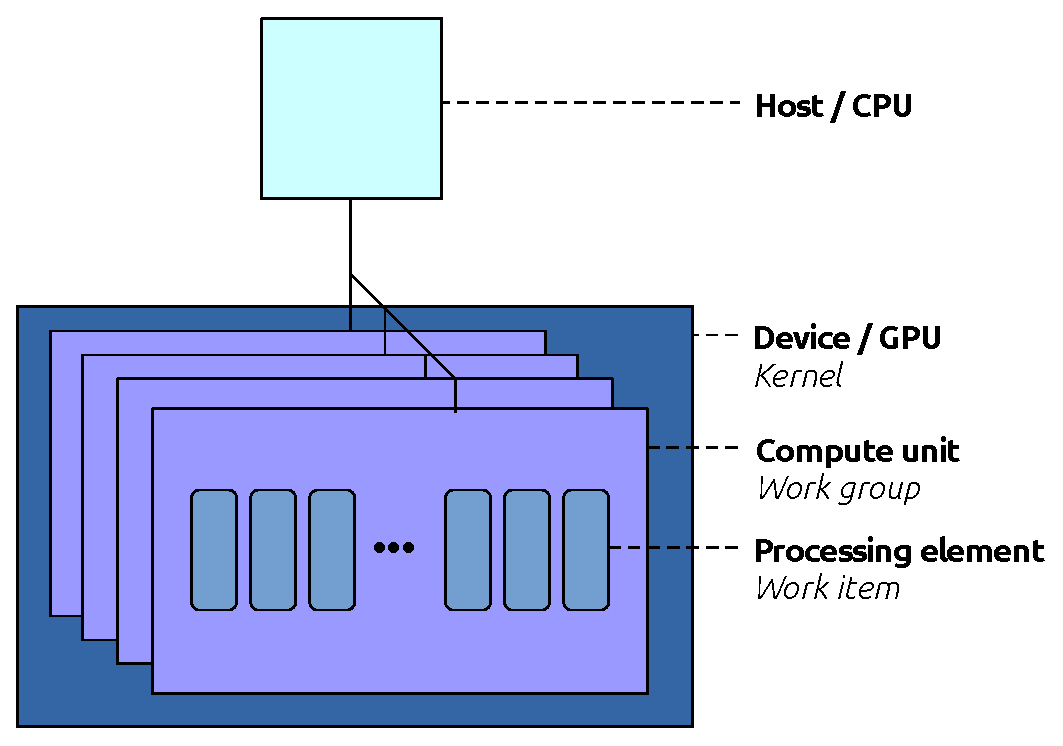
\includegraphics[width=2.5in]{resource/opencl_model.eps}
\caption{The OpenCL platform and execution model}
\label{fig:opencl}
\end{figure}

In the OpenCL platform and execution model (figure \ref{fig:opencl}), the user creates a host (in 
our case, the CPU) program that compiles and dispatches a GPGPU program to run on a particular 
device (the GPU).  Upon executing the kernel, the user must specify the number of work groups to 
execute as well as the size of each work group.  The execution model defines work items to be an 
executing instance of an OpenCL kernel which are run on processing elements, and work groups to be 
equally sized groups of work items. The OpenCL runtime ensures that work items within a work group 
will execute concurrently on the same compute unit, but provides no guarantees whether work items 
across work groups will execute concurrently or serially. All work items within a group are assigned 
a local id that is unique within that group as well as a global id that is unique across all work 
items in all work groups of the executing kernel.  The work items then make use of their local and 
global ids to appropriately divide up the work, and can make use of synchronization constructs like 
a work group barriers to synchronize their execution (but only for work items within the same group) 
\cite{opencl_guide}.

% An example of a floating figure using the graphicx package.
% Note that \label must occur AFTER (or within) \caption.
% For figures, \caption should occur after the \includegraphics.
% Note that IEEEtran v1.7 and later has special internal code that
% is designed to preserve the operation of \label within \caption
% even when the captionsoff option is in effect. However, because
% of issues like this, it may be the safest practice to put all your
% \label just after \caption rather than within \caption{}.
%
% Reminder: the "draftcls" or "draftclsnofoot", not "draft", class
% option should be used if it is desired that the figures are to be
% displayed while in draft mode.
%
%\begin{figure}[!t]
%\centering
%\includegraphics[width=2.5in]{myfigure}
% where an .eps filename suffix will be assumed under latex, and a .pdf suffix will be assumed for 
% pdflatex; or what has been declared
% via \DeclareGraphicsExtensions.
%\caption{Simulation Results}
%\label{fig_sim}
%\end{figure}

% Some.
% \begin{figure}[h]
% \centering
% \includegraphics[width=0.4\linewidth,angle=-90]{benchmarks/cache-scratch/cache-scratch.ps}
% \caption{Performance and scalability of allocators on threadtest}
% \label{fig:threadtest}
% \end{figure}

\section{Evaluation}

An existing implementation of an OpenCL kernel implementing the AES encryption algorithm was 
obtained from a public source code repository \cite{opencl_impl}.  The original implementation of 
the OpenCL encrypt kernel is implemented using a data parallel programming model, whereby a program 
is parallelized by performing the same computation on different pieces of data \cite{opencl_guide}.  
In particular, it only makes use of the global id of a work group to index itself into the input 
array at a particular position (e.g. index 0 of the input array), with one work group instance being 
responsible for encrypting an entry of the input array. The kernel also makes use of the vector 
instruction set of the GPU to increase the number of bytes that a single "entry" in the input array 
corresponds to. In particular, in addition to traditional analogs to C data types like 
$\mathtt{uint}$ (a 32-bit integer for a total of 4 bytes), there are vector data types like 
$\mathtt{uint4}$ (4 32-bit integers, for total of 16 bytes). Using these vector types allows one to 
execute native vector operations for the target platform \cite{opencl_guide}.  In particular, a 
single work item can operate on 16 bytes at once, whereas a traditional CPU would operate on 4 bytes 
at once. Thus, given an input array of $N$ bytes, we only need $N/16$ work groups of 1 work item 
each to encrypt an input array. Hence, in this implementation, the local id is ignored, since a work 
group only consists of a single work item.

The target device used for conducting experiments was a MotoX phone (table \ref{table:specs}).  We 
initially intended to use the Nexus 4 phone, but this was abandoned due to apparent instabilities 
triggered by the use of OpenCL on the device. 

Preliminary experiments determined that the full parallelism offered by the GPU was not being 
exploited using the original implementation.  Hence, modifications were made to the original 
implementation in order to explore the different levels of parallelism offered by varying the input 
parameters to the kernel such as the number of work groups and the work group size (which were 
previously strictly $N/16$ and 1 respectively).  The following sections describe the modifications 
that were performed to the original implementation and investigates their effect on the throughput 
of encryption.

\subsubsection{Version 1: even partitioning by work items}
\label{subsec:impl_partition}

We modified the OpenCL AES encrypt kernel such that the input array is split up evenly amongst the 
work items across all work groups (whereas previously they only encrypted 16 bytes). In particular, 
all OpenCL instances get some multiple of 16 bytes on which to operate, all of which are equally 
sized except one OpenCL instance which will be allocated whatever remains of the input array (i.e.  
given N = 128 bytes, and 3 work items, then 2 instances will operate on 48 bytes and 1 instance will 
operate on 32 bytes). Timing experiments were performed on a 128 MB input array, with the total 
number of work groups being varied from 1 up to 16, and the work group size being kept at 1 (refer 
to figure \ref{fig:num_work_groups}).

\begin{figure}[!t]
\centering
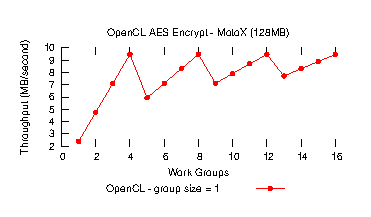
\includegraphics[width=2.5in]{../final/motox/4.2/sample_opencl_aes_global_worksize.128MB.16_max_global_worksize.again.report.eps}
\caption{OpenCL performance over a varying number of work groups}
\label{fig:num_work_groups}
\end{figure}

Going from of 1 up to 4 work groups, we see a linear speedup in encryption throughput (going from 
work groups of 1 to 2 we see a 2.37 MB/second speedup, 2 to 3 we see 2.36 MB/second, and 3 to 4 we 
see 2.36 MB/second). These linear speedups going from 1 up to 4 work groups are consistent with the 
device specifications in table \ref{table:specs} which state that the GPU has 4 computing units 
(hence, it is using an additional computing unit for each additional work group).

When we reach 5 work groups, we see the worst decrease in encryption throughput (3.54 MB/second).  
This is most likely due to the OpenCL runtime scheduling 4 simultaneous OpenCL kernel instances (4 
work groups each consisting of a single work item) that operate on $1/5$ of the input array, with a 
single OpenCL instance running on the remaining $1/5$ only after the first 4 complete (thereby 
underutilizing the parallelism of the GPU).

The throughput degrades the most for numbers of work groups that that are 1 modulo 4 since given 
that instances will tend to complete in roughly the same time (since they have the same data size 
and instructions executed), there will tend to be a point at which only one GPU core will be 
utilized, thus reducing parallelism (similarly for 2 modulo 4, and 3 modulo 4). As we increase the 
number of work groups, the degradation is less since the point at which we aren't maximally using 
all 4 GPU cores operates over less of the input array.  This phenomenon has been described in 
\cite{gpu_opt} as the tail effect.

Hence, from figure \ref{fig:num_work_groups}, the main conclusion to be drawn is that work groups 
are being scheduled on compute devices, but only one work group at a time is being scheduled 
(otherwise the peaks would reach above 10 MB/second as the number of work groups increases).

Next, we investigated the affect of increasing the number of work items used on a single compute 
device.  In particular, we began by querying the OpenCL runtime for the maximum available work group 
size, which was found to be 256.  However, this is only a theoretical maximum, and the actual 
maximum enforced by OpenCL is dependant on the kernel being executed and its resource requirements 
\cite{opencl_guide}; in our case, the maximum available was 80.  Timing experiments were performed 
on a 32 MB input array, with the total number of work items being varied from 1 up to 80, and the 
number of work groups being kept at 1 (refer to figure \ref{fig:work_group_size}).

\begin{figure}[!t]
\centering
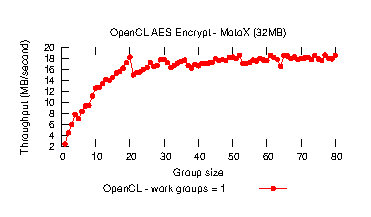
\includegraphics[width=2.5in]{../final/motox/4.2/sample_opencl_aes_work_group_size.32MB.1_work_groups.again.report.eps}
\caption{OpenCL performance over varying work group size}
\label{fig:work_group_size}
\end{figure}

From the graph, we can see the encryption throughput gradually increases from 0 up to 20 work items, 
doubling the maximum throughput observed when only considering a single work item (as in figure 
\ref{fig:num_work_groups}).  However, after 20 work items, we observe some degradation, followed by 
the throughput leveling off at around 18 MB/second in throughput.  This decrease in throughput for 
an increase in parallelism is an unexpected result and warranted further investigation.  Previous 
work has shown that the memory accesses patterns are important to consider when optimizing the 
performance of a GPU program \cite{gpu_mem}. In particular, access to global memory is the slowest 
memory operation, whereas access to local memory (shared within a work group) is more efficient 
\cite{opencl_guide}.  The current implementation would not benefit from the use of local memory for 
the input array since each work item reads global memory addresses once and encrypts it 
independently.  However, another important factor to consider is whether accesses to global memory 
within a warp \cite{gpu_mem} or team \cite{opencl_guide} (i.e. a hardware schedulable division of 
the work group size) are coalesced.  Memory accesses are said to be coalesced within a team if each 
work item in the team accesses global memory in an aligned, contiguous sequence of 32, 64, or 128 
bytes \cite{nvidia_opencl}. Hence, in the modification of the implementation in section 
\ref{subsec:impl_coalesce}, we investigate coalesced memory accesses.  

\subsubsection{GPU vs CPU Performance}
\label{subsec:gpu_vs_cpu}

Next, we evaluate the performance of encryption of the GPU over the CPU using the implementation in 
section \ref{subsec:impl_partition}.   Figure \ref{fig:num_work_groups} was used to guide selection 
of an optimal number of work groups (4) and figure \ref{fig:work_group_size} was used in choosing an 
optimal work group size (19).  The CPU implementation of AES encryption uses the OpenSSL crypto 
library \cite{openssl}, using a 256 bit AES key and CBC encryption mode.  In both the GPU and CPU 
implementations, timing measurements are restricted only to the encryption operation (i.e. not 
including any input initialization operations).  Timing experiments were performed on input sizes 
varying from 16 bytes up to 512 MB incrementing by powers of 2 (refer to figure 
\ref{fig:opencl_vs_cpu}).

\begin{figure}[!t]
\centering
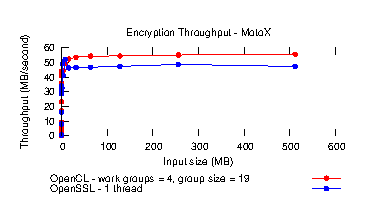
\includegraphics[width=2.5in]{../final/motox/4.2/opencl_sizes_vs_cpu_sizes.opencl_4G_19L.cpu_1thread.report.eps}
\caption{OpenCL GPU vs OpenSSL performance in AES encryption}
\label{fig:opencl_vs_cpu}
\end{figure}

From figure \ref{fig:opencl_vs_cpu}, we are able achieve a throughput of 55.68 MB/second at an input 
size of 512 MB, whereas the CPU is able to achieve 51.87 MB/second at an input size of 8 MB (though 
it quickly degrades to 46.25 MB/second for an input of 16 MB).  Hence, the GPU's overall increase in 
throughput speed is 3.81 MB/second over the CPU.  This margin is rather small based on previously 
published experiments investigating GPU encryption acceleration on the desktop (cite a paper). 
Hence, this result warranted further investigation into the implementation and potential 
optimizations.

\subsubsection{Version 2: coalesced accesses within work groups}
\label{subsec:impl_coalesce}

We further modified the kernel (from section \ref{subsec:impl_partition}) such that in addition to 
work items operating on equal sized input chunks, the work items within a work group access 
contiguous sequences.  

That is, the kernel in section \ref{subsec:impl_partition} performed strided memory accesses 
\cite{gpu_mem} within a work group.  For example, given a single work group of size 2 where each 
work item is responsible for encrypting $\mathtt{E}$ entries, the accesses to the input array 
$\mathtt{A}$ were as follows:

\begin{table}[h]
\centering
\begin{tabular}{ccc}
    \textbf{Work item 0} & \textbf{Work item 1} \\
    $\mathtt{A[i]}$         & $\mathtt{A[i + E]}$ \\
    $\mathtt{A[i + 1]}$     & $\mathtt{A[i + E + 1]}$ \\
    \ldots       & \ldots \\
    $\mathtt{A[i + E - 1]}$ & $\mathtt{A[i + 2*E - 1]}$ \\
\end{tabular}
\end{table}

In the following implementation, the memory accesses within such a work group have been modified 
such that instead of concurrent memory accesses being $\mathtt{E}$ entries apart, they are 
contiguous.  That is, if we have a total of $\mathtt{G}$ work groups, the accesses now look like:

\begin{table}[h]
\centering
\begin{tabular}{ccc}
    \textbf{Work item 0} & \textbf{Work item 1} \\
    $\mathtt{A[i]}$         & $\mathtt{A[i + 1]}$ \\
    $\mathtt{A[i + E]}$     & $\mathtt{A[i + 1 + E]}$ \\
    \ldots       & \ldots \\
    $\mathtt{A[i + E*(G - 1)]}$ & $\mathtt{A[i + 1 + E*(G - 1)]}$ \\
\end{tabular}
\end{table}

Timing experiments were performed on a 64 MB input array, with the total number of entries for a 
work item to encrypt being varied from 1 (16 bytes) up to 5000 (78K).  In order to fully utilize all 
potential processing power, the work group size was set to 80 and the number of work groups was set 
such that all 4 compute units were used (refer to figure \ref{fig:coalesce}).

\begin{figure}[!t]
\centering
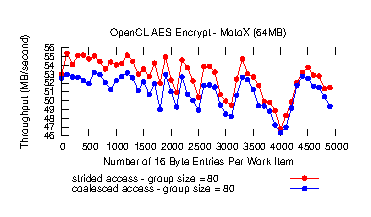
\includegraphics[width=2.5in]{../final/motox/4.2/sample_opencl_aes_entries.64MB.4_work_groups.5000_max_entries.both.eps}
\caption{OpenCL performance over for strided vs coalesced accesses within a work group}
\label{fig:coalesce}
\end{figure}

From figure \ref{fig:coalesce}, we generally achieve the best encryption throughput for a small 
number of entries ($< 500$), and it tends to get worse at the peaks for increasingly larger sizes 
per work item.  These drops in the peaks could be caused by increasingly large stride distances 
within a work group. 

The fluctuations observed in the graph are due to the GPU being underutilized near the end of the 
computation.  In particular, in order to use a work group size of 80, the OpenCL runtime forces the 
user to make each work group that size.  If the number of work items needed doesn't evenly divide 
the input, this will cause the final scheduled work groups to underutilize the GPU (and it becomes 
increasingly bad if a work item is responsible for a larger encryption size).

Comparing the coalesced and strided implementations, we observe nearly identical throughput 
behaviour.  However, we get slightly less throughput, which is likely due to the increased 
operations being performed for entry index calculations \cite{opencl_guide}.  However, if memory 
coalescing is in fact the reason for poor performance in the strided implementation, then the 
coalesced graph indicates that memory accesses are still not coalesced.  

This warrants further investigation into the memory access patterns for data other than the input 
array, such as the T-box lookup table which is used during the encryption process (cite AES).  In  
current implementations, this table is stored in constant memory (a constant region of global memory 
\cite{opencl_guide}) and may be subject to random uncoalesced accesses.

% Note that IEEE typically puts floats only at the top, even when this
% results in a large percentage of a column being occupied by floats.


% An example of a double column floating figure using two subfigures.
% (The subfig.sty package must be loaded for this to work.)
% The subfigure \label commands are set within each subfloat command, the
% \label for the overall figure must come after \caption.
% \hfil must be used as a separator to get equal spacing.
% The subfigure.sty package works much the same way, except \subfigure is
% used instead of \subfloat.
%
%\begin{figure*}[!t]
%\centerline{\subfloat[Case I]\includegraphics[width=2.5in]{subfigcase1}%
%\label{fig_first_case}}
%\hfil
%\subfloat[Case II]{\includegraphics[width=2.5in]{subfigcase2}%
%\label{fig_second_case}}}
%\caption{Simulation results}
%\label{fig_sim}
%\end{figure*}
%
% Note that often IEEE papers with subfigures do not employ subfigure
% captions (using the optional argument to \subfloat), but instead will
% reference/describe all of them (a), (b), etc., within the main caption.


% An example of a floating table. Note that, for IEEE style tables, the \caption command should come 
% BEFORE the table. Table text will default to
% \footnotesize as IEEE normally uses this smaller font for tables.
% The \label must come after \caption as always.
%
%\begin{table}[!t]
%% increase table row spacing, adjust to taste
%\renewcommand{\arraystretch}{1.3}
% if using array.sty, it might be a good idea to tweak the value of
% \extrarowheight as needed to properly center the text within the cells
%\caption{An Example of a Table}
%\label{table_example}
%\centering
%% Some packages, such as MDW tools, offer better commands for making tables
%% than the plain LaTeX2e tabular which is used here.
%\begin{tabular}{|c||c|}
%\hline
%One & Two\\
%\hline
%Three & Four\\
%\hline
%\end{tabular}
%\end{table}

\begin{table}[]
\centering
\caption{MotoX device specifications}
\label{table:specs}
\csvautotabular{resource/motox_specs.txt}
\end{table}



% Note that IEEE does not put floats in the very first column - or typically
% anywhere on the first page for that matter. Also, in-text middle ("here")
% positioning is not used. Most IEEE journals/conferences use top floats
% exclusively. Note that, LaTeX2e, unlike IEEE journals/conferences, places
% footnotes above bottom floats. This can be corrected via the \fnbelowfloat
% command of the stfloats package.

\section{Related work}
CleanOS is a modification of Android that introduces an abstraction called Sensitive Data Objects 
(SDOs) to track sensitive data on the RAM, created and hoarded by apps that run on top of the Dalvik 
Virtual Machine \cite{cleanos}. The system works by defining SDOs (either by the apps or by the default OS), 
which are a logical collection of Java Objects that contain sensitive data. It introduces a modified 
garbage collector known as EvictIdleGarbageCollector (eiGC) which walks through an idle SDO and 
encrypts their data-bearing fields using a key which is then evicted to the cloud whereas the data 
remains encrypted in memory.  This system, like ours, prevents the download delay of the encrypted 
data from a remote host as the data is always present in the device itself. Moreover, the key is 
inaccessible to a malicious user stealing the phone.

However, CleanOS incurs the latency of a network requests in retrieving the key from cloud.  In 
particular, CleanOS will incur unpredictable pauses during an otherwise inexpensive memory access on 
an encrypted value when the application is running due to network requests for obtaining keys from 
the cloud . Due to the implementation of encryption at the Davlik VM level, the application doesn't 
even have a means for knowing when the pauses are going to happen to prevent them either from doing 
something else in the meantime, or to avoid the request altogether.  In fact, evaluations show that 
many operations (like loading of an email onto the screen) incurred overheads of more than 100\% 
compared to a non-CleanOS implementation, especially over 3G networks \cite{cleanos}.

In contrast, our system stores the key on the device in a special register accessed by the operating 
system and not user level applications. We can use techniques like TRESOR \cite{tresor} for this, 
which ensures that the key is only stored in CPU registers which are not accessible to user 
applications (like debug registers) and that the key is only brought to RAM for a very short period 
on reboot even before all other applications come to life. The key is cleared from RAM soon after 
this.  Another major shortcoming of CleanOS is that it only encrypts data (memory) which is managed 
by the Dalvik virtual machine, and does not account for data that is unencrypted in other parts of 
the operating system \cite{cleanos}.  This includes OS data buffers (e.g. for writing to a file, 
inside device drivers from reading from sensors such as a camera).

XOM is a system to prevent software piracy, wherein the executing code of the software which is in 
RAM is encrypted by marking it as "execute-only" and so is prevented from tampering \cite{xom}. 
Cryptkeeper is a software-encrypted virtual memory manager that segments RAM into two segments, one 
for running the decrypted programming instructions (small in size) and the other for keeping the 
encrypted pages. The pages are swapped automatically between the segments and decrypted on demand 
\cite{cryptkeeper}.  Encrypted Swap aims at encrypting pages before swapping them to swap memory so 
that sensitive data related to swapped out processes are not available in backing storages 
\cite{encryptedswap}. These 
systems all have the same disadvantage that, even though the data is encrypted, the decryption key 
is still left in RAM and so can be recovered through memory-harvesting techniques.


\section{Conclusion}

In this report, we have taken the first steps in investigating the feasibility of using the GPU as a 
cryptographic accelerator for the AES algorithm on mobile devices.  In particular, our focus was on 
exploring the use of OpenCL as a framework for implementing the algorithm.  Using modifications of 
an existing implementation, we first showed that OpenCL schedules work groups to execute exclusively 
on the compute units of the GPU, and that optimal throughput must be achieved through more than just 
a simple data parallel implementation. Next, we investigated how performance varied with the 
implementation as the number of active work items a single compute unit was varied, discovering a 
surprising level off in encryption throughput when only using $\mathtt{1/4}$ of the available work 
items.  Next, we determined that using optimal parameters for the number of work groups and work 
group size, we are able to achieve on par performance with a single CPU using the OpenSSL 
implementation.  Finally, we investigated uncoalesced memory accesses in the input data as a 
potential reason for lower than expected performance, but determined this as not being the 
underlying cause.  

\section{Future work}

Our next endeavour would be to further investigate causes for reduced throughput in GPU encryption.  
In particular, we would investigate the affect of memory access patterns for data other than the 
input array, such as the T-box lookup table (see section \ref{subsec:impl_coalesce}).  Further, we 
would investigate the use of local memory regions shared between work items in a work group for 
accelerating redundant accesses to T-box values.  After achieving sufficient performance in 
encryption throughput, we would turn our focus to evaluating other characteristics relevant to 
mobile devices, such as energy consumption during encryption.  Finally, we would investigate methods 
for securely providing a privileged user-level process the permissions needed to encrypt memory on 
behalf of the Linux kernel.

% conference papers do not normally have an appendix


% trigger a \newpage just before the given reference
% number - used to balance the columns on the last page
% adjust value as needed - may need to be readjusted if
% the document is modified later
%\IEEEtriggeratref{8}
% The "triggered" command can be changed if desired:
%\IEEEtriggercmd{\enlargethispage{-5in}}

% references section

% can use a bibliography generated by BibTeX as a .bbl file
% BibTeX documentation can be easily obtained at:
% http://www.ctan.org/tex-archive/biblio/bibtex/contrib/doc/
% The IEEEtran BibTeX style support page is at:
% http://www.michaelshell.org/tex/ieeetran/bibtex/
%\bibliographystyle{IEEEtran}
% argument is your BibTeX string definitions and bibliography database(s)
%\bibliography{IEEEabrv,../bib/paper}
%
% <OR> manually copy in the resultant .bbl file
% set second argument of \begin to the number of references
% (used to reserve space for the reference number labels box)
% \begin{thebibliography}{1}
% 
% \bibitem{IEEEhowto:kopka}
% H.~Kopka and P.~W. Daly, \emph{A Guide to \LaTeX}, 3rd~ed.\hskip 1em plus
%   0.5em minus 0.4em\relax Harlow, England: Addison-Wesley, 1999.
% 
% \end{thebibliography}


\begin{filecontents*}{bibliography.bib}

    @misc{specs,
        title = {{PDAdb.net} Qualcomm Snapdragon S4 Pro MSM8960DT Multi-core Application Processor 
        with Modem Datasheet},
        howpublished = 
        {\url{http://www.pdadb.net/index.php?m=cpu&id=a8960dt&c=qualcomm_snapdragon_s4_pro_msm8960dt}},
        note = {Accessed: 2013-12-04}
    },

    @misc{gpu_opt,
        title = {{NVIDIA} GPU Performance Analysis and Optimization},
        howpublished = 
        {\url{http://on-demand.gputechconf.com/gtc/2012/presentations/S0514-GTC2012-GPU-Performance-Analysis.pdf}},
        note = {Accessed: 2013-12-04}
    },

    @misc{opencl_impl,
        title = {{GitHub} softboysxp/OpenCL-AES},
        howpublished = {\url{https://github.com/softboysxp/OpenCL-AES}},
        note = {Accessed: 2013-12-04}
    },

    @misc{nvidia_opencl,
        title = {{NVIDIA} OpenCL Programming Guide for the CUDA Architecture},
        howpublished = 
        {\url{http://www.nvidia.com/content/cudazone/download/OpenCL/NVIDIA_OpenCL_ProgrammingGuide.pdf}},
        note = {Accessed: 2013-12-04}
    },

    @book{opencl_guide,
        title={OpenCL programming guide},
        author={Munshi, Aaftab and Gaster, Benedict and Mattson, Timothy G and Ginsburg, Dan},
        year={2011},
        publisher={Pearson Education}
    }

    @inproceedings{gpu_mem,
        title={A GPGPU compiler for memory optimization and parallelism management},
        author={Yang, Yi and Xiang, Ping and Kong, Jingfei and Zhou, Huiyang},
        booktitle={ACM Sigplan Notices},
        volume={45},
        number={6},
        pages={86--97},
        year={2010},
        organization={ACM}
    }

    @misc{openssl,
        title = {{OpenSSL} Documents, crypto(3)},
        howpublished = {\url{http://www.openssl.org/docs/crypto/crypto.html}},
        note = {Accessed: 2013-12-04}
    },

    @article{coldboot,
        title={Lest we remember: cold-boot attacks on encryption keys},
        author={Halderman, J Alex and Schoen, Seth D and Heninger, Nadia and Clarkson, William and Paul, William and Calandrino, Joseph A and Feldman, Ariel J and Appelbaum, Jacob and Felten, Edward W},
        journal={Communications of the ACM},
        volume={52},
        number={5},
        pages={91--98},
        year={2009},
        publisher={ACM}
    },

    @inproceedings{tresor,
        title={TRESOR Runs Encryption Securely Outside RAM},
        author={M{\"u}ller, Tilo and Freiling, Felix C and Dewald, Andreas},
        booktitle={USENIX Security Symposium},
        year={2011}
    },

    @article{myth,
        title={CPU and/or GPU: Revisiting the GPU Vs. CPU Myth},
        author={Kothapalli, Kishore and Banerjee, Dip Sankar and Narayanan, PJ and Sood, Surinder and 
            Bahl, Aman Kumar and Sharma, Shashank and Lad, Shrenik and Singh, Krishna Kumar and Matam, Kiran 
        and Bharadwaj, Sivaramakrishna and others},
        journal={arXiv preprint arXiv:1303.2171},
        year={2013}
    },

    @inproceedings{aes_gpu,
        title={Accelerating Encryption Algorithms Using Parallelism},
        author={Duta, Cristina-Loredana and Michiu, Gicu and Stoica, Silviu and Gheorghe, Laura},
        booktitle={Control Systems and Computer Science (CSCS), 2013 19th International Conference on},
        pages={549--554},
        year={2013},
        organization={IEEE}
    },

    @inproceedings{cleanos,
        title={CleanOS: Limiting mobile data exposure with idle eviction},
        author={Tang, Yang and Ames, Phillip and Bhamidipati, Sravan and Bijlani, Ashish and Geambasu, 
        Roxana and Sarda, Nikhil},
        booktitle={Proceedings of the USENIX Conference on Operating Systems Design and Implementation, 
        Berkeley, CA, USA},
        year={2012}
    },

    @article{xom,
        title={Architectural support for copy and tamper resistant software},
        author={Lie, David and Thekkath, Chandramohan and Mitchell, Mark and Lincoln, Patrick and Boneh, Dan and Mitchell, John and Horowitz, Mark},
        journal={ACM SIGPLAN Notices},
        volume={35},
        number={11},
        pages={168--177},
        year={2000},
        publisher={ACM}
    },

    @inproceedings{cryptkeeper,
        title={Cryptkeeper: Improving security with encrypted RAM},
        author={Peterson, Peter AH},
        booktitle={Technologies for Homeland Security (HST), 2010 IEEE International Conference on},
        pages={120--126},
        year={2010},
        organization={IEEE}
    },

    @inproceedings{encryptedswap,
        title={Encrypting virtual memory},
        author={Provos, Niels},
        booktitle={Proceedings of the Ninth USENIX Security Symposium},
        pages={35--44},
        year={2000}
    },

    @article{aes1,
        title={197, Advanced encryption standard (AES)},
        author={FIPS, PUB},
        journal={National Institute of Standards and Technology},
        year={2001}
    }

    @misc{aes2,
        title={The Design of Rijndael: AES-The Advanced Encryption Standard (Information Security and Cryptography)},
        author={Daemen, Joan and Rijmen, Vincent},
        year={2002},
        publisher={Springer Heidelberg}
    }

\end{filecontents*}

% \newpage
\bibliographystyle{plain}
\bibliography{bibliography}

% that's all folks
\end{document}
